\documentclass[conference]{IEEEtran}
\IEEEoverridecommandlockouts
% The preceding line is only needed to identify funding in the first footnote. If that is unneeded, please comment it out.
\usepackage{cite}
\usepackage{amsmath}
\usepackage{amsmath,amssymb,amsfonts}
\usepackage{algorithmic}
\usepackage{graphicx}
\usepackage{textcomp}
\usepackage{xcolor}
\def\BibTeX{{\rm B\kern-.05em{\sc i\kern-.025em b}\kern-.08em
    T\kern-.1667em\lower.7ex\hbox{E}\kern-.125emX}}
\begin{document}

\title{CMSC 603 of Fall-2021 : High-Performance Distributed Systems\\Report on Assignment-2
% {\footnotesize}
}

\author{\IEEEauthorblockN{Md Touhiduzzaman}
\IEEEauthorblockA{\textit{Department of Computer Science} \\
\textit{Virginia Commonwealth University (VCU)}\\
Richmond, Virginia, USA \\
touhiduzzamm@vcu.edu}
}

\maketitle

\begin{abstract}
In this assignment, the impact of multiple threads, MPI and CUDA are tested on an implementation of the kNN algorithm. Firstly, the performance of the kNN algorithm is measured for a single threaded implementation and then tested respectively with multi-threaded, OpenMP, MPI and CUDA implementations for 1, 2, 4, 8, 16, 32, 64, 128 and 256 threads. In general, it is observed that the threaded versions continue to run faster roughly till the limit of the number of available processes in the host machine and then the runtimes again get worse due to the overheads of threaded operations like communication, forks and join. Depending on the efficiency and effectiveness of the implementations, the results comply with this concept.
Then CUDA kernel is used to test the algorithm with different threads. A significant improvement on the runtime as well as dataset-size independent runtime is seen using CUDA, but a fall in accuracy is seen.
\end{abstract}

\begin{IEEEkeywords}
threads, openmp, mpi, knn, cuda
\end{IEEEkeywords}


\section{Methodology}
Posix thread is used to implement the multi-threaded version. The dataset is evenly distributed for each thread by calculating the partition size from the avaialabe data points and the number of available threads. The threads are joined to combine the predictions. Besides, OpenMP is used to implement further parallel version of the algorithm to let others to be compared as per their runtime and accuracy.
Then, a CUDA kernel is defined to predict the class of the test instances. This kernel is run for various number of threads as 1, 2, 4, 8, 16, 32, 64, 128 and 256 threads like other versions of the code. For the CUDA kernel call, the block count is calculated as per the division of the test-cases in between the defined number of threads. The formula used here is - for $numTestInstances$ number of test-instances and $numThreads$ number of threads, the number of blocks, \[numBlocks=\textstyle\frac{numTestInstances ~ + ~ numThreads ~ - ~ 1}{numThreads} \]
The algorithms are run in the Maple VM of VCU having 28 processes.\\
There were 3 sample datasets tested in the given assignment - a small-dataset with 592 training data and 80 test data, a medium sized dataset with 7354 training data and 370 test data and another large dataset with 30803 training data and 1718 test data. The results found from all of these 3 are discussed in the following section \ref{res}.

\section{Results}\label{res}

\subsection{Small Dataset}
The sequential code requires 7 milliseconds to deliver 85\% accurate predictions. But the versions of openmp and MPI implementations require much less time to deliver similar or more accurate data. In contrary, the CUDA version requires almost a constant amount of time around \textit{670 ms} with a much less accuracy of 58.75\%. 
\ref{tab:Table1} represents the collected runtime-data and ``Fig.~\ref{fig1}'' shows the runtime-graph for all the 5 methods using 1,2,4,8,16,32,64,128 and 256 threads on the small data set. The accuracy of the runs is represented by the Table~\ref{tab:Table2} and Fig.~\ref{fig2}.

\begin{table}
    \begin{tabular}{||c | c | c | c | c | c||} 
     \hline
     Threads & Sequential & Multithreaded & OpenMP & MPI & CUDA \\ [0.2ex] 
     \hline\hline
     1	& 7	& 7	& 7 & 7 & 688\\ 
     \hline
    2 & 7 & 4 & 3 & 7 & 667\\
     \hline
    4 & 7 & 6 & 2 & 7 & 665\\
     \hline
    8 & 7 & 6 & 1 & 7 & 671\\
     \hline
    16 & 7 & 7& 1 & 7 & 665\\ [1ex] 
     \hline
    32 & 7 & 10 & 2 & 7 & 687\\ [1ex] 
     \hline
    64 & 7 & 12 & 2 & 7 & 667 \\ [1ex] 
     \hline
    128 & 7 & 13 & 4 & 7 & 669 \\ [1ex] 
     \hline
    256 & 7 & 12 & 5 & 7 & 657 \\ [1ex] 
     \hline
    \end{tabular}
\caption{\label{tab:Table1}Runtime for Small Dataset}
\end{table}

\begin{figure}[htbp]
    \centerline{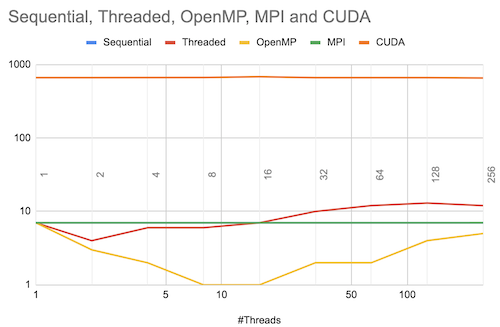
\includegraphics{report/rt_small_set.png}}
    \caption{Runtimes for Small Dataset}
    \label{fig1}
\end{figure}

\begin{table}
    \begin{tabular}{||c | c | c | c | c | c||} 
     \hline
     Threads & Sequential & Multithreaded & OpenMP & MPI & CUDA \\ [0.2ex] 
     \hline\hline
    1 & 85 & 85 & 85 & 85 & 58.75\\ [1ex] 
     \hline
    2 & 85 & 86.25 & 85 & 85 & 58.75\\ [1ex] 
     \hline
    4 & 85 & 85 & 85 & 85 &  58.75\\ [1ex] 
     \hline
    8 & 85 & 85 & 85 & 85 & 58.75\\ [1ex] 
     \hline
    16 & 85 & 85 & 85 & 85 & 58.75\\ [1ex] 
     \hline
    32 & 85 & 85 & 85 & 85 & 58.75\\ [1ex] 
     \hline
    64 & 85 & 85 & 85 & 85 & 58.75\\ [1ex] 
     \hline
    128 & 85 & 85 & 85 & 85 & 58.75\\ [1ex] 
     \hline
    256 & 85 & 85 & 85 & 85 & 58.75\\ [1ex] 
     \hline
    \end{tabular}
\caption{\label{tab:Table2}Accuracy for Small Dataset}
\end{table}

\begin{figure}[htbp]
\centerline{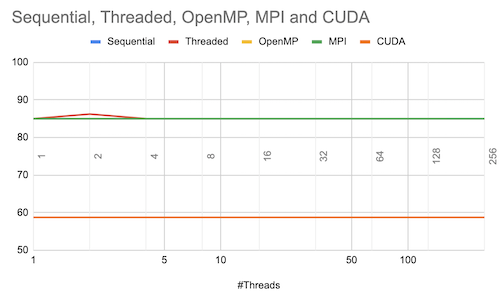
\includegraphics{report/acc_small_set.png}}
\caption{Accuracy for Small Dataset}
\label{fig2}
\end{figure}

\subsection{Medium Dataset}
The sequential code requires around 600 milliseconds to deliver 25.95\% accurate predictions. But the multi-threaded version requires lesser time for the increasing number of threads until 1, 2, 4 and 8, but it increases monotonically till the 256 number of threads. The OpenMP implementation requires lesser time for increasing number of threads. But, the CUDA implementation requires almost similar runtime as the small-data set, i.e., around 620 ms for a very low accuracy rate of 8.65\%. 
Table~\ref{tab:Table3} and Table~\ref{tab:Table4} show the runtime and accuracy of the different implementations, while the Fig.~\ref{fig3} and Fig.~\ref{fig4} show their corresponding graphical presentations.

\begin{table}
    \begin{tabular}{||c | c | c | c | c | c||} 
     \hline
     Threads & Sequential & Multithreaded & OpenMP & MPI & CUDA \\ [0.2ex] 
     \hline\hline
    1 & 629	& 610 & 604 & 629	& 698\\ [1ex] 
     \hline
    2 & 628	& 309 & 311 & 628	& 669\\ [1ex] 
     \hline
    4 & 599	& 318 & 170 & 599	& 674\\ [1ex] 
     \hline
    8 & 597 & 475 & 87 & 597	& 699\\ [1ex] 
     \hline
    16 & 596 & 609 & 73 & 596	& 676\\ [1ex] 
     \hline
    32 & 596 & 776 & 39 & 596	& 669\\ [1ex] 
     \hline
    64 & 630 & 926 & 40 & 630 & 677\\ [1ex] 
     \hline
    128 & 627 & 1127 & 41 & 627 & 695\\ [1ex] 
     \hline
    256 & 627 & 1155 & 29 & 627 & 699\\ [1ex] 
     \hline
    \end{tabular}
\caption{\label{tab:Table3}Runtime for Medium Dataset}
\end{table}

\begin{figure}[htbp]
\centerline{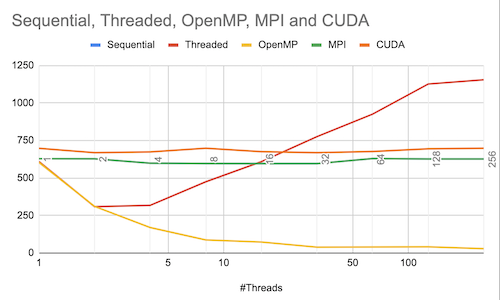
\includegraphics{report/rt_medium_set.png}}
\caption{Runtimes for Medium Dataset}
\label{fig3}
\end{figure}

\begin{table}
    \begin{tabular}{||c | c | c | c | c | c||} 
    \hline
    Threads & Sequential & Multithreaded & OpenMP & MPI & CUDA \\ [0.2ex] 
    \hline\hline
    1 & 85 & 85 & 85 & 85 & 8.65\\ [1ex] 
    \hline
    2 & 85 & 86.25 & 85 & 85 & 8.65\\ [1ex] 
    \hline
    4 & 85 & 85 & 85 & 85 & 8.65\\ [1ex] 
    \hline
    8 & 85 & 85 & 85 & 85 & 8.65\\ [1ex] 
    \hline
    16 & 85 & 85 & 85 & 85 & 8.65\\ [1ex] 
     \hline
    32 & 85 & 85 & 85 & 85 & 8.65\\ [1ex] 
     \hline
    64 & 85 & 85 & 85 & 85 & 8.65\\ [1ex] 
     \hline
    128 & 85 & 85 & 85 & 85 & 8.65\\ [1ex] 
     \hline
    256 & 85 & 85 & 85 & 85 & 8.65\\ [1ex] 
     \hline
    \end{tabular}
\caption{\label{tab:Table4}Accuracy for Medium Dataset}
\end{table}

\begin{figure}[htbp]
    \centerline{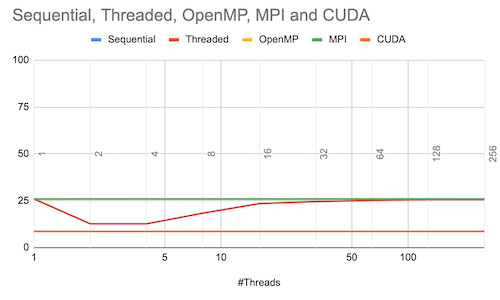
\includegraphics{report/acc_medium_set.png}}
    \caption{Accuracy for Medium Dataset}
    \label{fig4}
\end{figure}

\subsection{Large Dataset}
The sequential code requires around 1200 milliseconds to deliver 99.48\% accurate predictions. But the multi-threaded version requires lesser time for the increasing number of threads until 1, 2 and 4, but it increases monotonically till the 256 number of threads. The OpenMP implementation requires lesser time for increasing number of threads. But, the CUDA implementation requires almost similar runtime around 740 ms for a very low accuracy rate of 8.96\%. 
Table~\ref{tab:Table5} and Table~\ref{tab:Table6} show the runtime and accuracy of the different implementations, while the Fig.~\ref{fig5} and Fig.~\ref{fig6} show their corresponding graphical presentations.

\begin{table}
    \begin{tabular}{||c | c | c | c | c | c||} 
     \hline
     Threads & Sequential & Multithreaded & OpenMP & MPI & CUDA \\ [0.2ex] 
     \hline\hline
    1 & 11973 & 12121 & 11982 & 11973 & 977 \\ [.1ex] 
     \hline
    2 & 12030 & 6576 & 6509 & 12030 & 782 \\ [.1ex] 
     \hline
    4 & 11980 & 6477 & 3258 & 11980 & 730 \\ [.1ex] 
     \hline
    8 & 12009 & 9533 & 1786 & 12009 & 736 \\ [.1ex] 
     \hline
    16 & 11996 & 11624 & 1068 & 11996 & 719 \\ [.1ex] 
     \hline
    64 & 12116 & 16599 & 642 & 12116 & 720 \\ [.1ex] 
     \hline
    128 & 11906 & 20225 & 495 & 11906 & 743 \\ [.1ex] 
     \hline
    256 & 12233 & 38863 & 485 & 12233 & 743 \\ [.1ex] 
     \hline
    \end{tabular}
\caption{\label{tab:Table5}Runtimes for Large Dataset}
\end{table}

\begin{figure}[htbp]
    \centerline{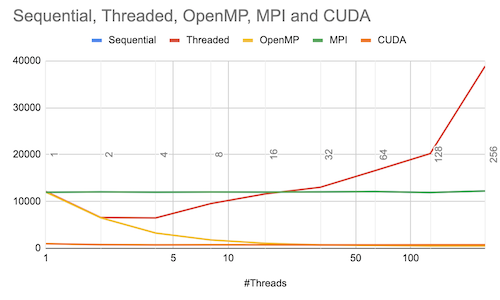
\includegraphics{report/rt_large_set.png}}
    \caption{Runtimes for Large Dataset}
    \label{fig5}
\end{figure}


\begin{table}
    \begin{tabular}{||c | c | c | c | c | c||} 
     \hline
     Threads & Sequential & Multithreaded & OpenMP & MPI & CUDA \\ [0.1ex] 
     \hline\hline
    1 & 99.48 & 99.48 & 99.48 & 99.48 & 8.96 \\ [.1ex] 
     \hline
    2 & 99.48 & 50.06 & 99.48 & 99.48 & 8.96 \\ [.1ex] 
     \hline
    4 & 99.48 & 50.06 & 99.48 & 99.48 & 8.96 \\ [.1ex] 
     \hline
    8 & 99.48 & 75.09 & 99.48 & 99.48 & 8.96 \\ [.1ex] 
     \hline
    16 & 99.48 & 87.6 & 99.48 & 99.48 & 8.96 \\ [.1ex] 
     \hline
    32 & 99.48 & 93.83 & 99.48 & 99.48 & 8.96 \\ [.1ex] 
     \hline
    64 & 99.48 & 96.97 & 99.48 & 99.48 & 8.96 \\ [.1ex] 
     \hline
    128 & 99.48 & 98.54 & 99.48 & 99.48 & 8.96 \\ [.1ex] 
     \hline
    256 & 99.48 & 99.3 & 99.48 & 99.48 & 8.96 \\ [.1ex] 
     \hline
    \end{tabular}
\caption{\label{tab:Table6}Accuracy for Large Dataset}
\end{table}

\begin{figure}[htbp]
    \centerline{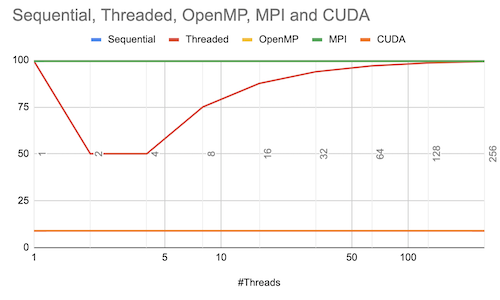
\includegraphics{report/acc_large_set.png}}
    \caption{Accuracy for Large Dataset}
    \label{fig6}
\end{figure}

\begin{figure}[htbp]
    \centerline{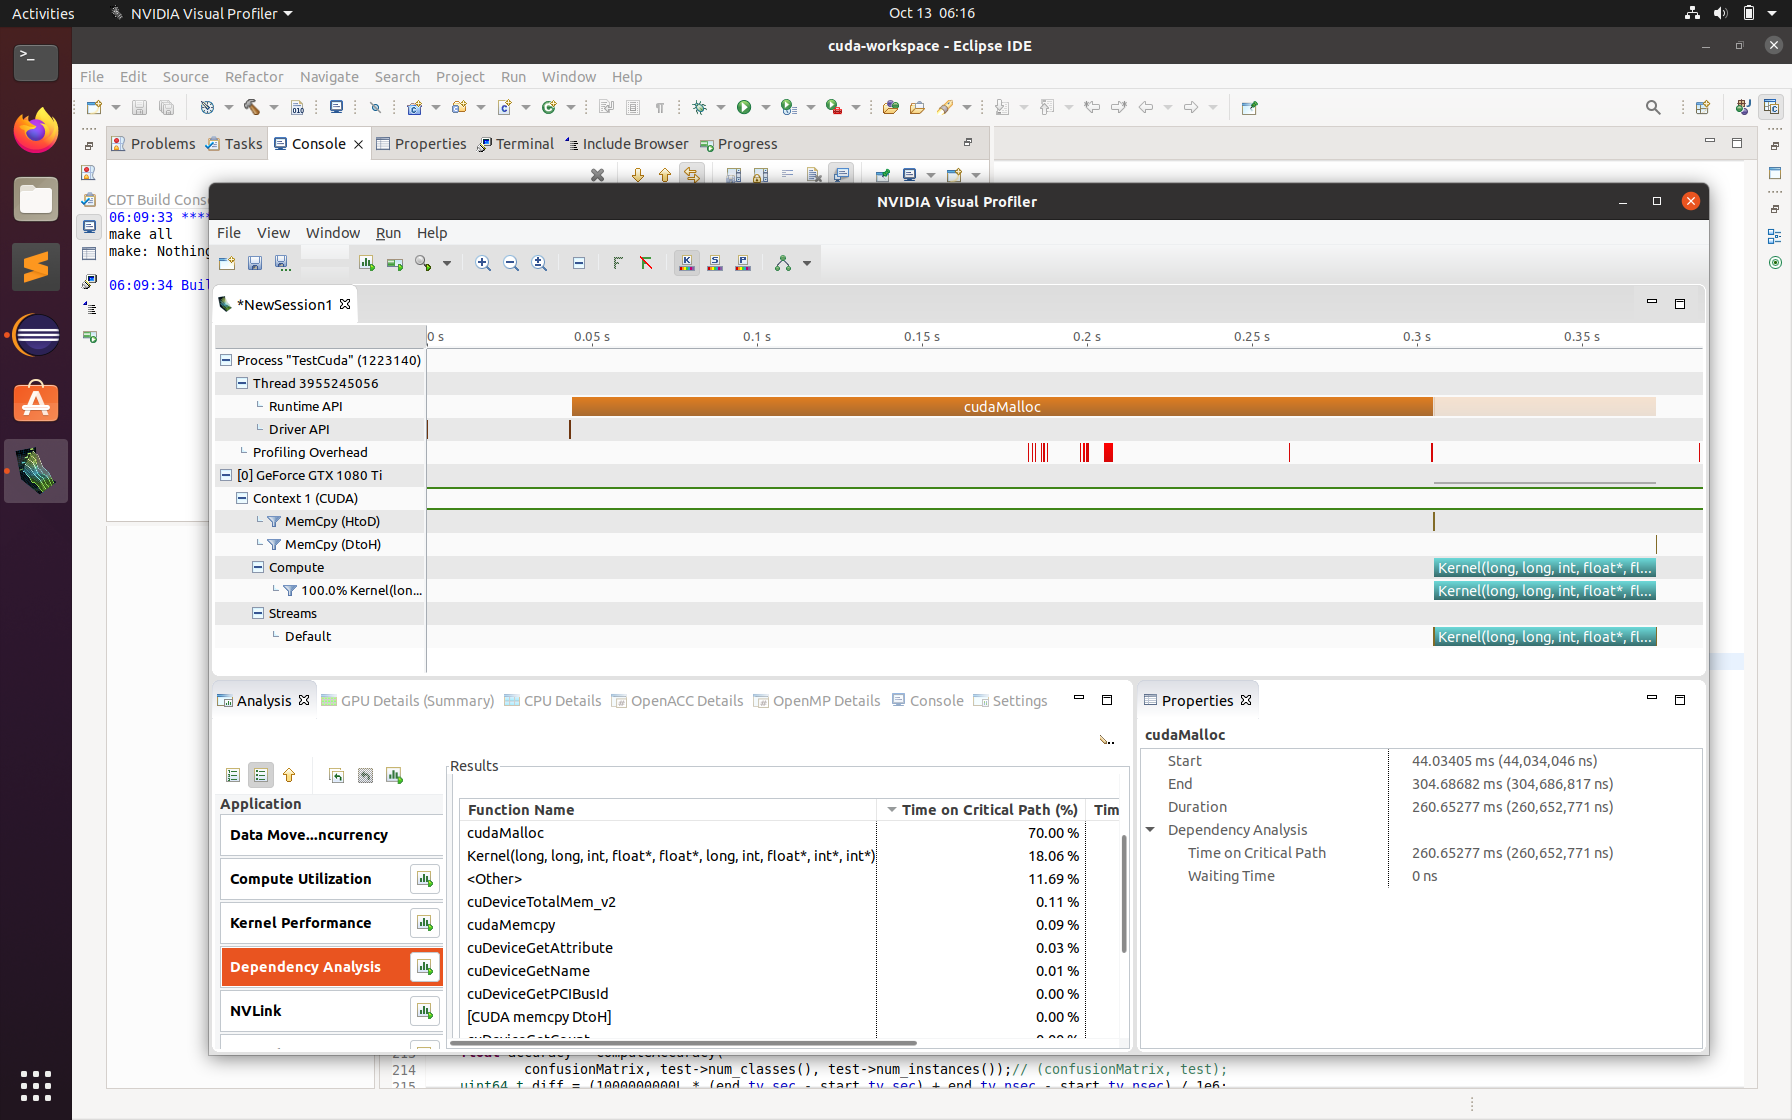
\includegraphics[width=1\linewidth]{report/profiler.png}}
    \caption{Eclipse Profiler Screenshot for CUDA Kernel execution}
    \label{fig7}
\end{figure}


\subsection{Speedup and Scalability Analysis}
From the profiler analysis in Eclipse for the CUDA run of 256 threads, we can get that the \textit{cudaMalloc} operation requires the maximum sequential time of 260.67 milliseconds, while the Kernel calls require 67.27 milliseconds on average and other sequential processes accumulate to around 44.5 milliseconds. Here, we can say that the total runtime of the CUDA code for 256 threads is 372.44 ms and that of the serial execution is 12233 ms. So, the scalability of the CUDA implementation in comparison to the sequential code is 33 times.

\section*{Conclusion}
The multithreaded code actually has a few misconfigurations to deliver worse runtime than the sequential version of the implementation, though it is theoretically to be correct after the available processes, i.e. 28 in the Maple server, is exceeded by the 32 to 256 number of threads' runs. About the CUDA runtime, it can be said that the memory operations require the major portion of the runtime and, that being universal for any number of threads and almost identical for any length of the memory operation due to the large bandwidth between the host and the device, it is requiring very minor fluctuation due to the size of the data-set and almost no fluctuation for different number of threads. This judgement can be verified from the Fig.~\ref{fig7} showing the Eclipse profiler screenshot, where the \textit{cudaMalloc} operations are seen to consume more than 70\% of the total runtime for a 256 thread-per-block run of the CUDA implementation.


\begin{thebibliography}{00}
\bibitem{b1} Dr. Alberto Cano, Slides and lecture notes for ``CMSC-603 (High Performance and Distributed Systems`` course of fall-2021, Virginia Commonwealth University, Richmond, VA.

\bibitem{b2} Fayez Gebali, ``Algorithms and Parallel Computing``.
\end{thebibliography}
\vspace{12pt}

\end{document}
